\documentclass[a4paper,11pt]{report}
\usepackage{chuan_math_gkt}
\usetikzlibrary{angles,quotes,intersections,patterns,decorations.pathreplacing}
\chuanexamsetup

\begin{document}
\examfontsize

\examsecret{绝密$\bigstar$启用前}

\examtitle{2023年普通高等学校招生全国统一考试（天津卷）}{数\quad 学}

\noticetitle
\begin{examnotice}
\item 答卷前，考生务必将自己的姓名、准考证号填写在答题卡上。
\item 回答选择题时，选出每小题的答案后，用铅笔把答题卡上对应题目的答案标号涂黑。如需改动，用橡皮擦干净后，再选涂其他答案标号。回答非选择题时，将答案写在答题卡上。写在本试卷上无效。
\item 考试结束后，将本试卷和答题卡一并交回。
\end{examnotice}

\examsection{一、选择题：本大题共9小题，每小题5分，共45分。在每小题给出的四个选项中，只有一项是符合题目要求的。}
\begin{examquestions}

\item 已知集合 $U=\{1,2,3,4,5\}$，$A=\{1,3\}$，$B=\{1,2,4\}$，则 $\complement_U B\cup A=$
\fourchoices{$\{1,3,5\}$}{$\{1,3\}$}{$\{1,2,4\}$}{$\{1,2,4,5\}$}
\item “$a^2=b^2$”是“$a^2+b^2=2ab$”的
\twochoices{充分不必要条件}{必要不充分条件}{充要条件}{既不充分又不必要条件}
\item 若 $a=1.01^{0.5}$，$b=1.01^{0.6}$，$c=0.6^{0.5}$，则 $a,b,c$ 的大小关系为
\fourchoices{$c>a>b$}{$c>b>a$}{$a>b>c$}{$b>a>c$}
\item 函数 $f(x)$ 的图象如下图所示，则 $f(x)$ 的解析式可能为
\begin{tightcenter}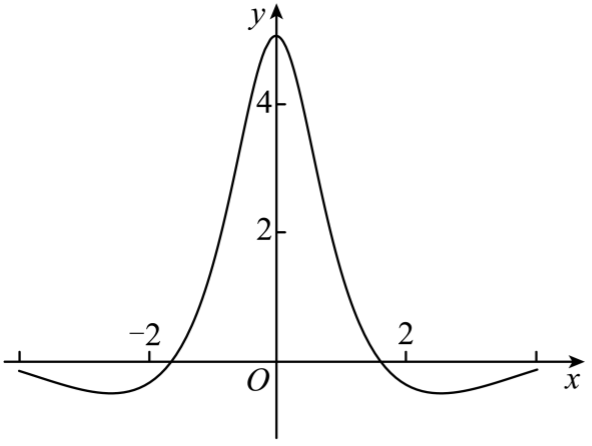
\includegraphics[width=5.5cm]{figures/2023_tj_q4.png}\end{tightcenter}
\fourchoices{\tallchoice{$\dfrac{5(e^x-e^{-x})}{x^2+2}$}}{\tallchoice{$\dfrac{5\sin x}{x^2+1}$}}{\tallchoice{$\dfrac{5(e^x+e^{-x})}{x^2+2}$}}{\tallchoice{$\dfrac{5\cos x}{x^2+1}$}}
\item 已知函数 $f(x)$ 的一条对称轴为直线 $x=2$，一个周期为 $4$，则 $f(x)$ 的解析式可能为
\fourchoices{$\sin\left(\dfrac\pi2x\right)$}{$\cos\left(\dfrac\pi2x\right)$}{$\sin\left(\dfrac\pi4x\right)$}{$\cos\left(\dfrac\pi4x\right)$}
\item 已知 $\{a_n\}$ 为等比数列，$S_n$ 为数列 $\{a_n\}$ 的前 $n$ 项和，$a_{n+1}=2S_n+2$，则 $a_4$ 的值为
\fourchoices{$3$}{$18$}{$54$}{$152$}
\item 调查某种群花萼长度和花瓣长度，所得数据如图所示，其中相关系数 $r=0.8245$，下列说法正确的是
\begin{tightcenter}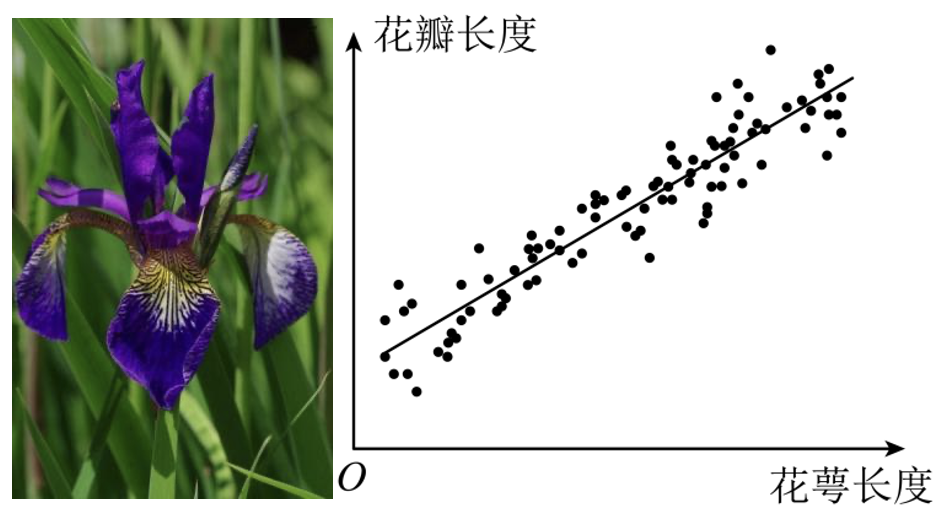
\includegraphics[width=7.6cm]{figures/2023_tj_q7.png}\end{tightcenter}
\onechoices{花瓣长度和花萼长度没有相关性}{花瓣长度和花萼长度呈现负相关}{花瓣长度和花萼长度呈现正相关}{若从样本中抽取一部分，则这部分的相关系数一定是 $0.8245$}
\item 在三棱锥 $P-ABC$ 中，线段 $PC$ 上的点 $M$ 满足 $PM=\dfrac13PC$，线段 $PB$ 上的点 $N$ 满足 $PN=\dfrac23PB$，则三棱锥 $P-AMN$ 和三棱锥 $P-ABC$ 的体积之比为
\fourchoices{\tallchoice{$\dfrac19$}}{\tallchoice{$\dfrac29$}}{\tallchoice{$\dfrac13$}}{\tallchoice{$\dfrac49$}}
\item 双曲线 $\dfrac{x^2}{a^2}-\dfrac{y^2}{b^2}=1(a>0,b>0)$ 的左、右焦点分别为 $F_1,F_2$。过 $F_2$ 作其中一条渐近线的垂线，垂足为 $P$。已知 $PF_2=2$，直线 $PF_1$ 的斜率为 $\dfrac{\sqrt2}{4}$，则双曲线的方程为
\fourchoices{\tallchoice{$\dfrac{x^2}{8}-\dfrac{y^2}{4}=1$}}{\tallchoice{$\dfrac{x^2}{4}-\dfrac{y^2}{8}=1$}}{\tallchoice{$\dfrac{x^2}{4}-\dfrac{y^2}{2}=1$}}{\tallchoice{$\dfrac{x^2}{2}-\dfrac{y^2}{4}=1$}}

\end{examquestions}

\examsection{二、填空题：本大题共6小题，每小题5分，共30分。试题中包含两个空的，答对1个的给3分，全部答对的给5分。}
\begin{examquestions}[start=10]

\item 已知 $\mathrm{i}$ 是虚数单位，化简 $\dfrac{5+14\mathrm{i}}{2+3\mathrm{i}}$ 的结果为\blank。
\item 在 $\left(2x^3-\dfrac1x\right)^6$ 的展开式中，$x^2$ 项的系数为\blank。
\item 过原点 $O$ 的一条直线与圆 $C:(x+2)^2+y^2=3$ 相切，交曲线 $y^2=2px(p>0)$ 于点 $P$，若 $|OP|=8$，则 $p$ 的值为\blank。
\newpage
\item 甲乙丙三个盒子中装有一定数量的黑球和白球，其总数之比为 $5:4:6$。这三个盒子中黑球占总数的比例分别为 $40\%,25\%,50\%$。现从三个盒子中各取一个球，取到的三个球都是黑球的概率为\blank；将三个盒子混合后任取一个球，是白球的概率为\blank。
\item 在 $\triangle ABC$ 中，$\angle A=60^\circ$，$BC=1$，点 $D$ 为 $AB$ 的中点，点 $E$ 为 $CD$ 的中点，若设 $\overrightarrow{AB}=\vec a$，$\overrightarrow{AC}=\vec b$，则 $\overrightarrow{AE}$ 可用 $\vec a,\vec b$ 表示为\blank；若 $\overrightarrow{BF}=\dfrac13\overrightarrow{BC}$，则 $\overrightarrow{AE}\cdot\overrightarrow{AF}$ 的最大值为\blank。
\item 若函数 $f(x)=ax^2-2x-|x^2-ax+1|$ 有且仅有两个零点，则 $a$ 的取值范围为\blank。

\end{examquestions}

\examsection{三、解答题：本大题共5小题，共75分。解答应写出文字说明、证明过程或演算步骤。}
\begin{examanswers}[start=16]

\item（14分）

在 $\triangle ABC$ 中，角 $A,B,C$ 所对边分别是 $a,b,c$。已知 $a=\sqrt{39}$，$b=2$，$\angle A=120^\circ$。

（1）求 $\sin B$ 的值；

（2）求 $c$ 的值；

（3）求 $\dfrac{\sin(B-C)}{\sin B}$。

\item（15分）

三棱台 $ABC-A_1B_1C_1$ 中，若 $AA_1\perp$ 面 $ABC$，$AB\perp AC$，$AB=AC=AA_1=2$，$A_1C_1=1$，$M,N$ 分别是 $BC,BA$ 中点。

\noindent\begin{minipage}[t]{0.64\linewidth}
（1）求证：$A_1N\parallel$ 平面 $C_1MA$；

（2）求平面 $C_1MA$ 与平面 $ACC_1A_1$ 所成夹角余弦值；

（3）求点 $C$ 到平面 $C_1MA$ 的距离。
\end{minipage}\hfill
\begin{minipage}[t]{0.3\linewidth}
\vspace{-2.0em}\centering
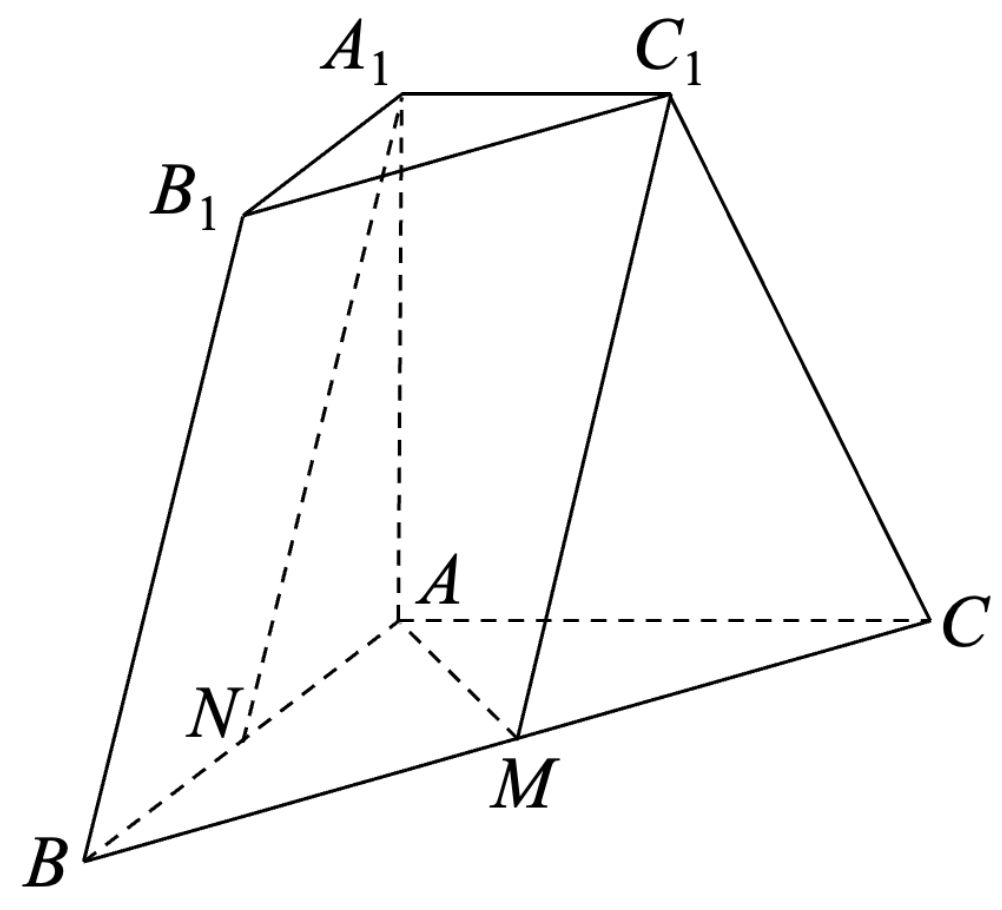
\includegraphics[width=\linewidth]{figures/2023_tj_q17.png}
\end{minipage}

\item（15分）

设椭圆 $\dfrac{x^2}{a^2}+\dfrac{y^2}{b^2}=1(a>b>0)$ 的左右顶点分别为 $A_1,A_2$，右焦点为 $F$，已知 $|A_1F|=3$，$|A_2F|=1$。

（1）求椭圆方程及其离心率；

（2）已知点 $P$ 是椭圆上一动点（不与端点重合），直线 $A_2P$ 交 $y$ 轴于点 $Q$，若三角形 $A_1PQ$ 的面积是三角形 $A_2FP$ 面积的二倍，求直线 $A_2P$ 的方程。

\item（15分）

已知 $\{a_n\}$ 是等差数列，$a_2+a_5=16$，$a_5-a_3=4$。

（1）求 $\{a_n\}$ 的通项公式和 $\displaystyle\sum_{i=2^{n-1}}^{2^n-1}a_i$。

（2）已知 $\{b_n\}$ 为等比数列，对于任意 $k\in\mathbb N^*$，若 $2^{k-1}\leq n\leq2^k-1$，则 $b_k<a_n<b_{k+1}$，

（1）当 $k\geq2$ 时，求证：$2^k-1<b_k<2^k+1$；

（2）求 $\{b_n\}$ 的通项公式及其前 $n$ 项和。

\item（16分）

已知函数 $f(x)=\left(\dfrac1x+\dfrac12\right)\ln(x+1)$。

（1）求曲线 $y=f(x)$ 在 $x=2$ 处切线的斜率；

（2）当 $x>0$ 时，证明：$f(x)>1$；

（3）证明：$\dfrac56<\ln(n!)-\left(n+\dfrac12\right)\ln n+n\leq1$。

\end{examanswers}

\end{document}
